\newpage
\section{Estimating the hydraulic conductivity drop in the rhizosphere} \label{sec:hydro_rhizo}
The resolution of the soil grid is often too coarse to catch small-scale rhizosphere gradients in hydraulic conductivity near the roots. The consequence is that root water uptake is overestimated. One solution would be (adaptive) grid refinement, however at the cost of computation time and the validity of the line-source assumption that we take for the roots in our setup. 
An alternative solution is to keep the coarse soil grid resolution and estimate the soil water potential at the root-soil interface. We implemented two ways of doing so within dumux-rosi. Firstly, we split the volume of each soil control element between the root segments that lie inside it, and assign a soil cylinder around each root segment. In each soil cylinder, the 1D radially symmetric Richards equation is solved and coupled to the macroscopic scale in a mass conservative way via the outer boundary conditions of the soil cylinders. 

\subsection{The steady-rate approximation}
The second approach is described in this example and follows the approach described in \cite{Schroeder2008}. Each root segment inside a soil control element of volume $V_s$ has an assigned ``rhizosphere soil volume" equal to $$V_{rhizo} = k V_s,$$ where the weighting factor $k$ is the fraction of the root segment volume $V_{rs}$ relative to the overall volume of roots $V_{rst\textsc{}}$ inside $V_s$, $k=\frac{V_{rs}}{V{rst}}$. 
From this, the outer radius of the rhizosphere cylinder is computed by 
$$r_{out}=\sqrt{\frac{V_{rhizo}+V_{rs}}{\pi l}},$$ where $l$ is the root segment length. 


Then the flux at the root-soil interface is estimated based on the analytical solutions of the 1D radially symmetric Richards equation. Based on the steady-rate assumption and using the matric flux potential $\Phi(h_c)=\int_{-\infty}^{h_c}  K(h) dh$ that linearizes the Richards equation, the radial matric flux potential profiles for non-stressed and stressed conditions are given by 
\begin{multline}
\Phi(r)=\Phi_{r_{out}} + (q_{root}r_{root}-q_{out}r_{out})\left[ \frac{r^2/r_{root}^2}{2(1-\rho^2)} + \frac{\rho^2}{1-\rho^2}\left(\text{ln}  \frac{r_{out}}{r}-\frac{1}{2} \right) \right] \\\ + q_{out}r_{out} \text{ln} \frac{r}{r_{out}}
\end{multline}
and 
\begin{multline}
\Phi(r) = \left(\Phi_{r_{out}} - \Phi_{r_{root}} + q_{out}r_{out}\text{ln} \frac{1}{\rho}\right)\frac{r^2/r_{root}^2 - 1 + 2\rho^2 \text{ln}  r_{root}/r}{\rho^2 -1 + 2\rho^2 ln 1/\rho} \\\ + q_{out}r_{out}\text{ln} \frac{r}{r_{root}} + \Phi_{root},
\end{multline}
where $\rho=\frac{r_{out}}{r_{root}}$, $r_{root}$ is the root radius, $r_{out}$ is the outer radius, $q_{root}$ is the flux prescribed at the root-soil interface, $q_{out}$ is the flux at the outer boundary.

Given the soil matric potential at the outer boundary, and either the flux (non-stressed conditions) or soil matric potential (stressed) at the root-soil interface, the solution computes the radial matrix flux potential profile, and from the matric flux potential, the soil matric potential can be inferred. The soil matric potential at the outer boundary is taken to be the macroscopic soil matric potential value of the given soil control element at the given time step. The water flux at the outer boundary, $q_{out}$, is computed such that the sum of the fluxes at the outer boundaries of the rhizosphere cylinders is equal to the net flux into or out of the given soil control element, $q_{V_s}$, at a given time step, and $$q_{out}=k q_{V_s}$$, where $k$ is the same weighting factor as described above. However, setting the outer flux to zero is sufficient in most cases, as there is redistribution after every time step.  

We start the simulation by computing the root water uptake according to the classical (see section \ref{s:coupling}). 
Then, for every root segment and at every time step, we check whether the matric flux potential at the root-soil interface is positive or negative. In case the matric flux potential is positive, root water uptake follows non-stressed conditions, and the sink term is left according to the classical approach. In case the matric flux potential is negative, root water uptake follows stressed conditions and the soil matric potential at the root-soil interface is equal to the wilting point. The water flux from soil into the root is computed by numerically approximating the soil matric potential gradient at the root-soil interface and multiplying this by the hydraulic conductivity.

Finally, the flux at the root-soil interface is the maximum of the classical and steady-rate approximation value. This makes sure that hydraulic redistribution (i.e. flow from roots to soil) is still possible. 

Listing X shows the code of file ``coupled_c12_schroeder.py".
%\lstinputlisting[firstline=1, language=Python, caption=Example 6a]{../../examples/python/example6a_mapping.py}

\begin{itemize}
\item[106-110] Root xylem potentials are computed based on the current soil (at first call) or rhizosphere (from second call onwards) water potentials. 
\item[112] Rhizosphere soil water potentials are updated from the current soil and xylem water potentials using the steady-rate assumption. 
\item[113] For each root segment, the water fluxes are computed from the current xylem and rhizosphere water potentials. 
\item[115] For the soil control element, sum of root water uptake over all root segments inside a given soil control element is computed. 
\item[127] The fluxes are set as sources in the soil problem (Richards equation)
\item[131] Soil problem is solved for one time step. 
\end{itemize}

   
Listing Y shows the C++ code for the computation of matric potential at the root-soil interface according to Schröder. The fluxes are then computed according to the pressure differences...
%\lstinputlisting[firstline=1, language=Python, caption=Example 6a]{../../examples/python/example6a_mapping.py}

\begin{itemize}
\item[234] Computation of the matrix flux potential according to the non-stressed equation. 
\item[237] For positive mfp (no stress), the soil matric potential at the root-soil interface is set to the corresponding value.
\item[240] For negative mfp (stress), the soil matric potential at the root-soil interface is set equal to the wilting point. 
\item[245] If the xylem water potential is larger than the root-soil interface potential, root-soil interface potential is set equal to the xylem water potential (no flux). 
\item[248] On the macroscopic scale, flow of water from root to soil is enabled. 
\end{itemize}


Figure \ref{fig:schroeder} the transpiration rate and cumulative transpiration computed based on the steady-rate assumption for the case of a clay soil. 
%
\begin{figure}
%\begin{subfigure}[c]{1\textwidth}
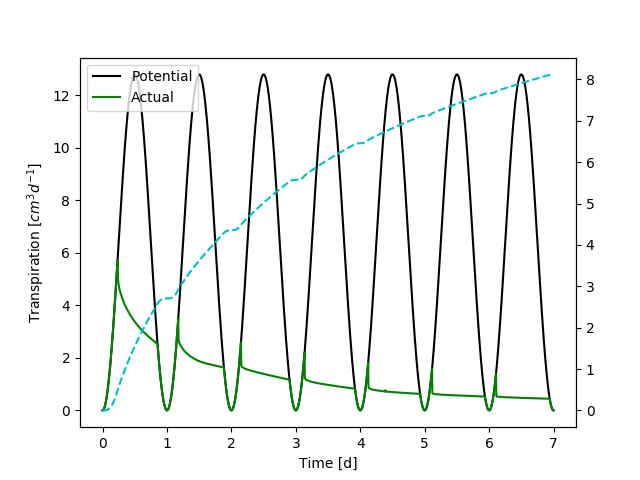
\includegraphics[width=0.99\textwidth]{clay_schroeder.png}
%\subcaption{Gravi- and Plagiotropism} \label{fig:example7c}
%\end{subfigure}
%\begin{subfigure}[c]{1\textwidth}
%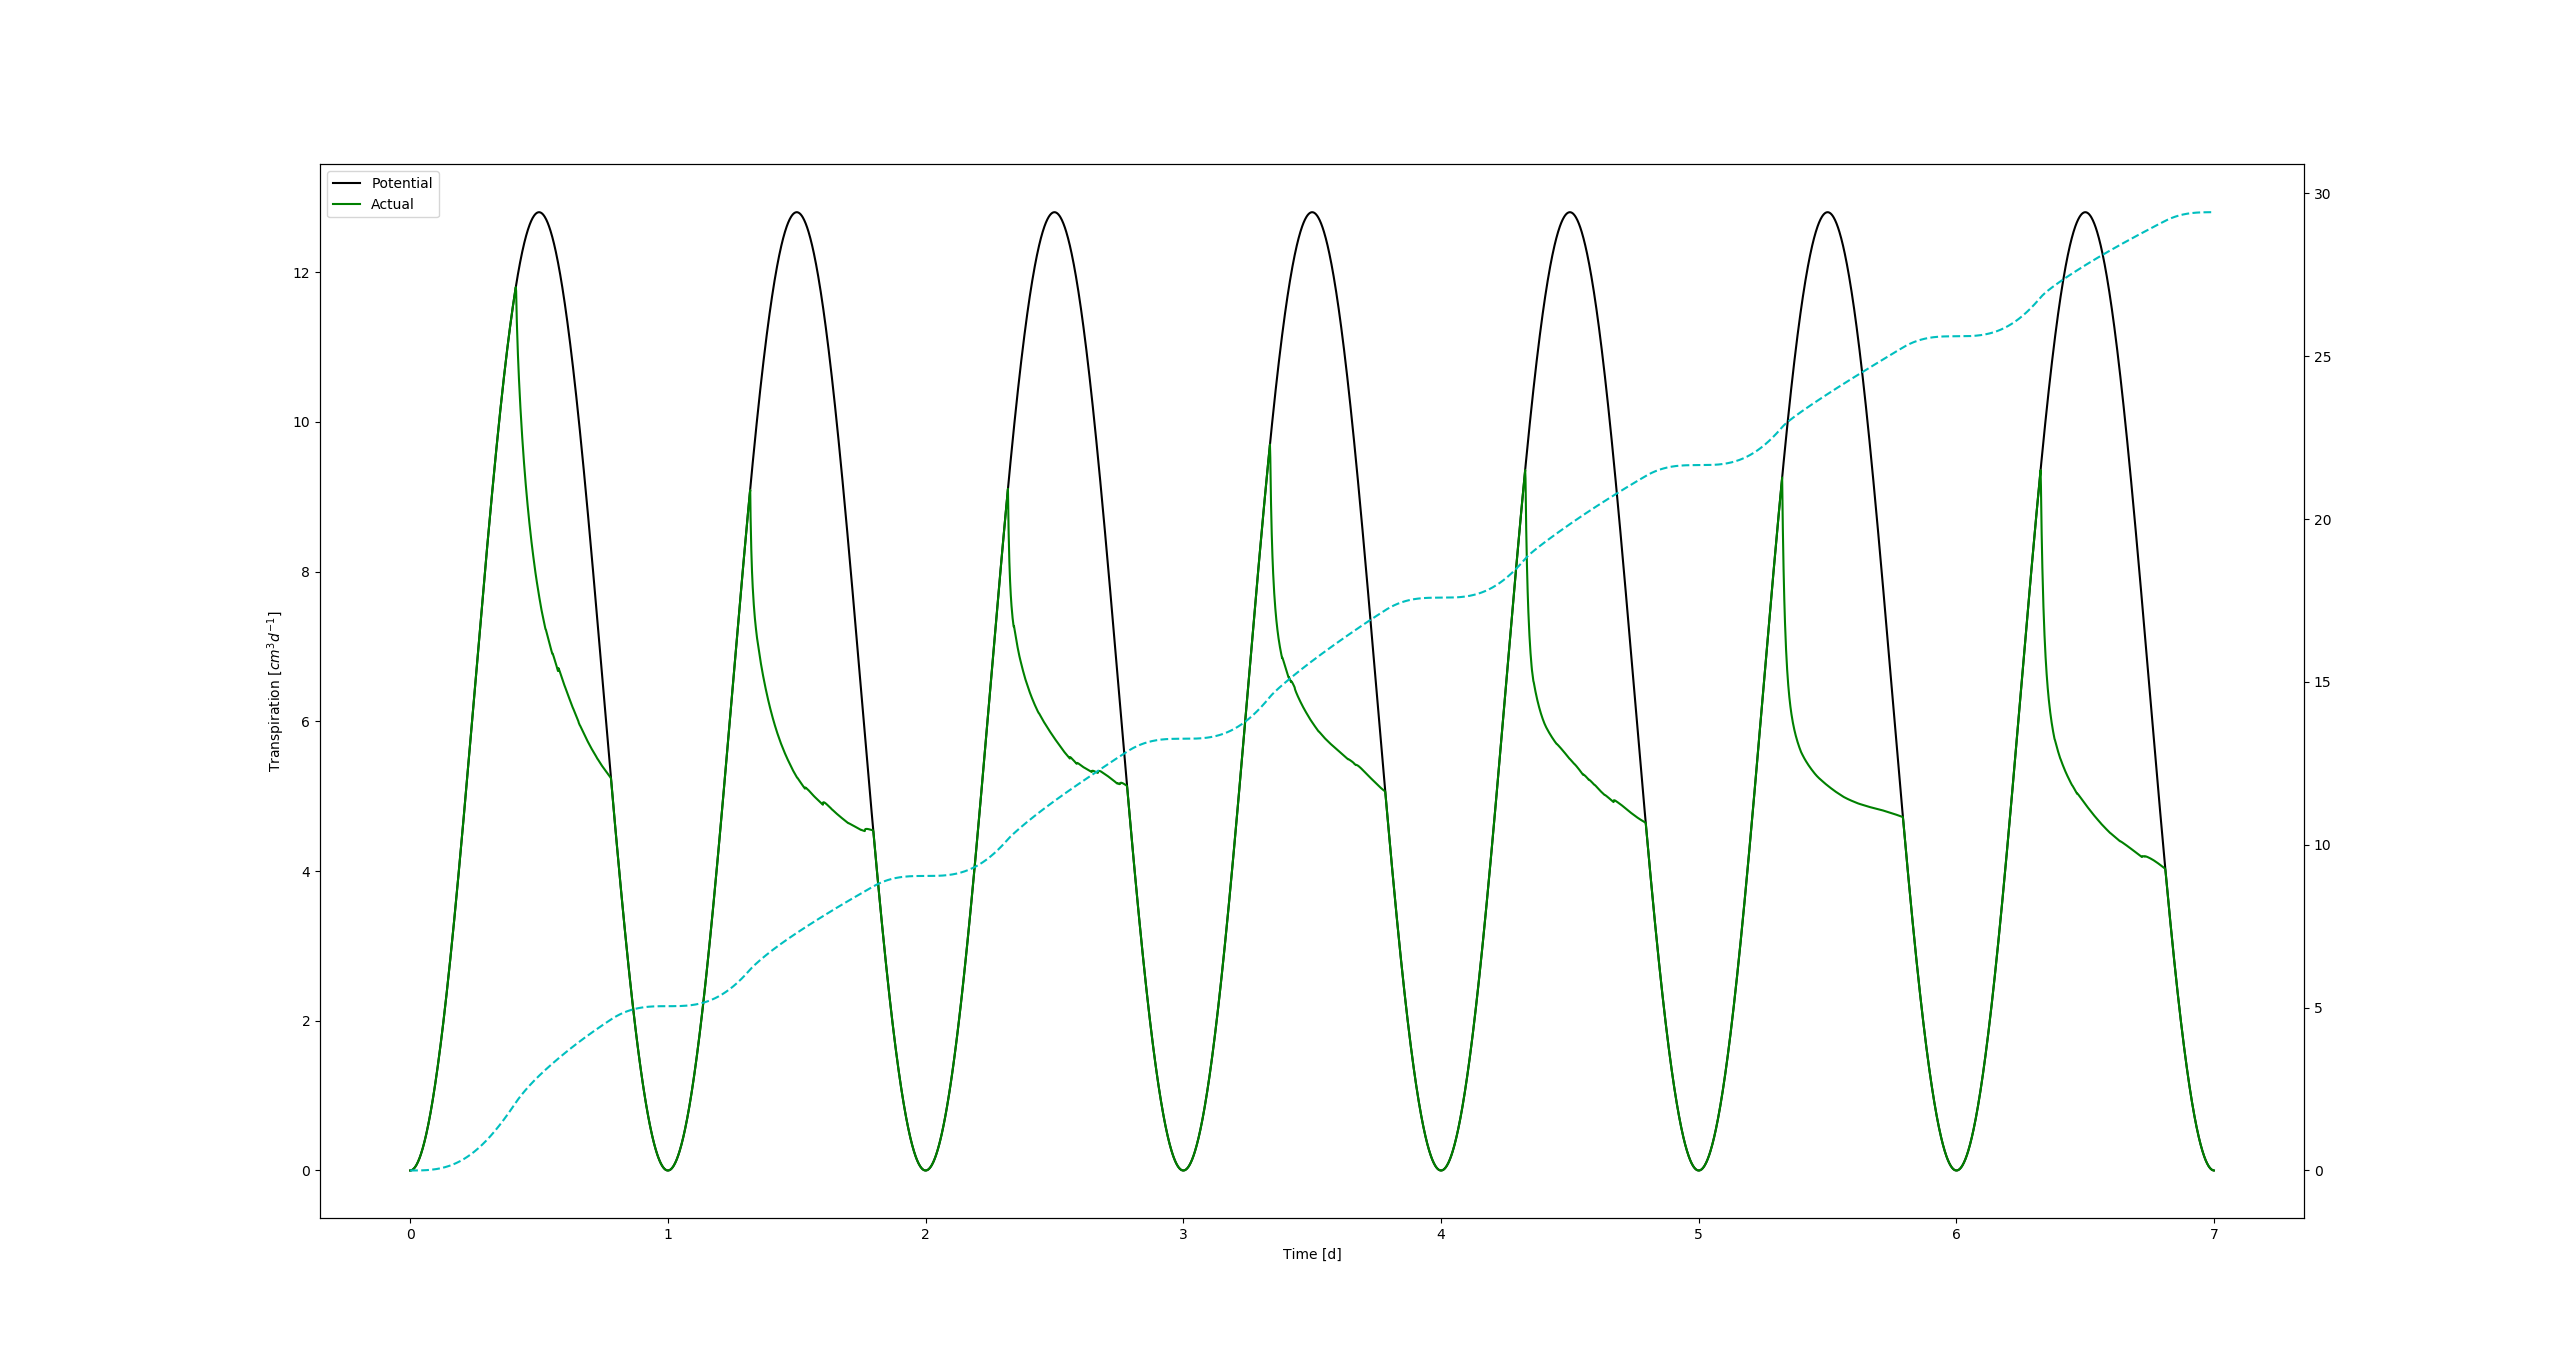
\includegraphics[width=0.99\textwidth]{example7c_simple_hydro.png}
%\subcaption{Hydrotropism} \label{fig:example7c_hydro}
%\end{subfigure}
\caption{Transpiration rate and cumulative transpiration computed based on the steady-rate assumption.} \label{fig:schroeder}
\end{figure}




